\chapter{Documenti}
\label{chap:Documenti}
In questa sezione, vengono riportati alcuni documenti che riguardano la costituzione della nostra Parrocchia:

\begin{itemize}
\item \textbf{Lettera fondazionale}: Convenzione tra Diocesi di Trieste e Provincia Patavina dei frati minori conventuali.
\item \textbf{Riconoscimento civile}: Lettera della prefettura che accoglie la richiesta dell Diocesi per riconoscere a livello civile la nuova Parrocchia.
\item \textbf{Saluto del Vescovo}: L'augurio del Vescovo Santin.
\end{itemize}

%\newpage\mbox{}\newpage
\newpage
\phantomsection
\addcontentsline{toc}{section}{Lettera fondazionale}
\markright{Lettera fondazionale}{}
\foreachpage{testi/lettera_fondazionale.pdf}{%
  \newpage   
  \begingroup 
    \centering
    \includegraphics[
      page=\value{imagepage},
      width=\textwidth,  
      height=\textheight,
    ]{testi/lettera_fondazionale.pdf}%
    \newpage
  \endgroup
}

%\newpage
%\begin{center}
%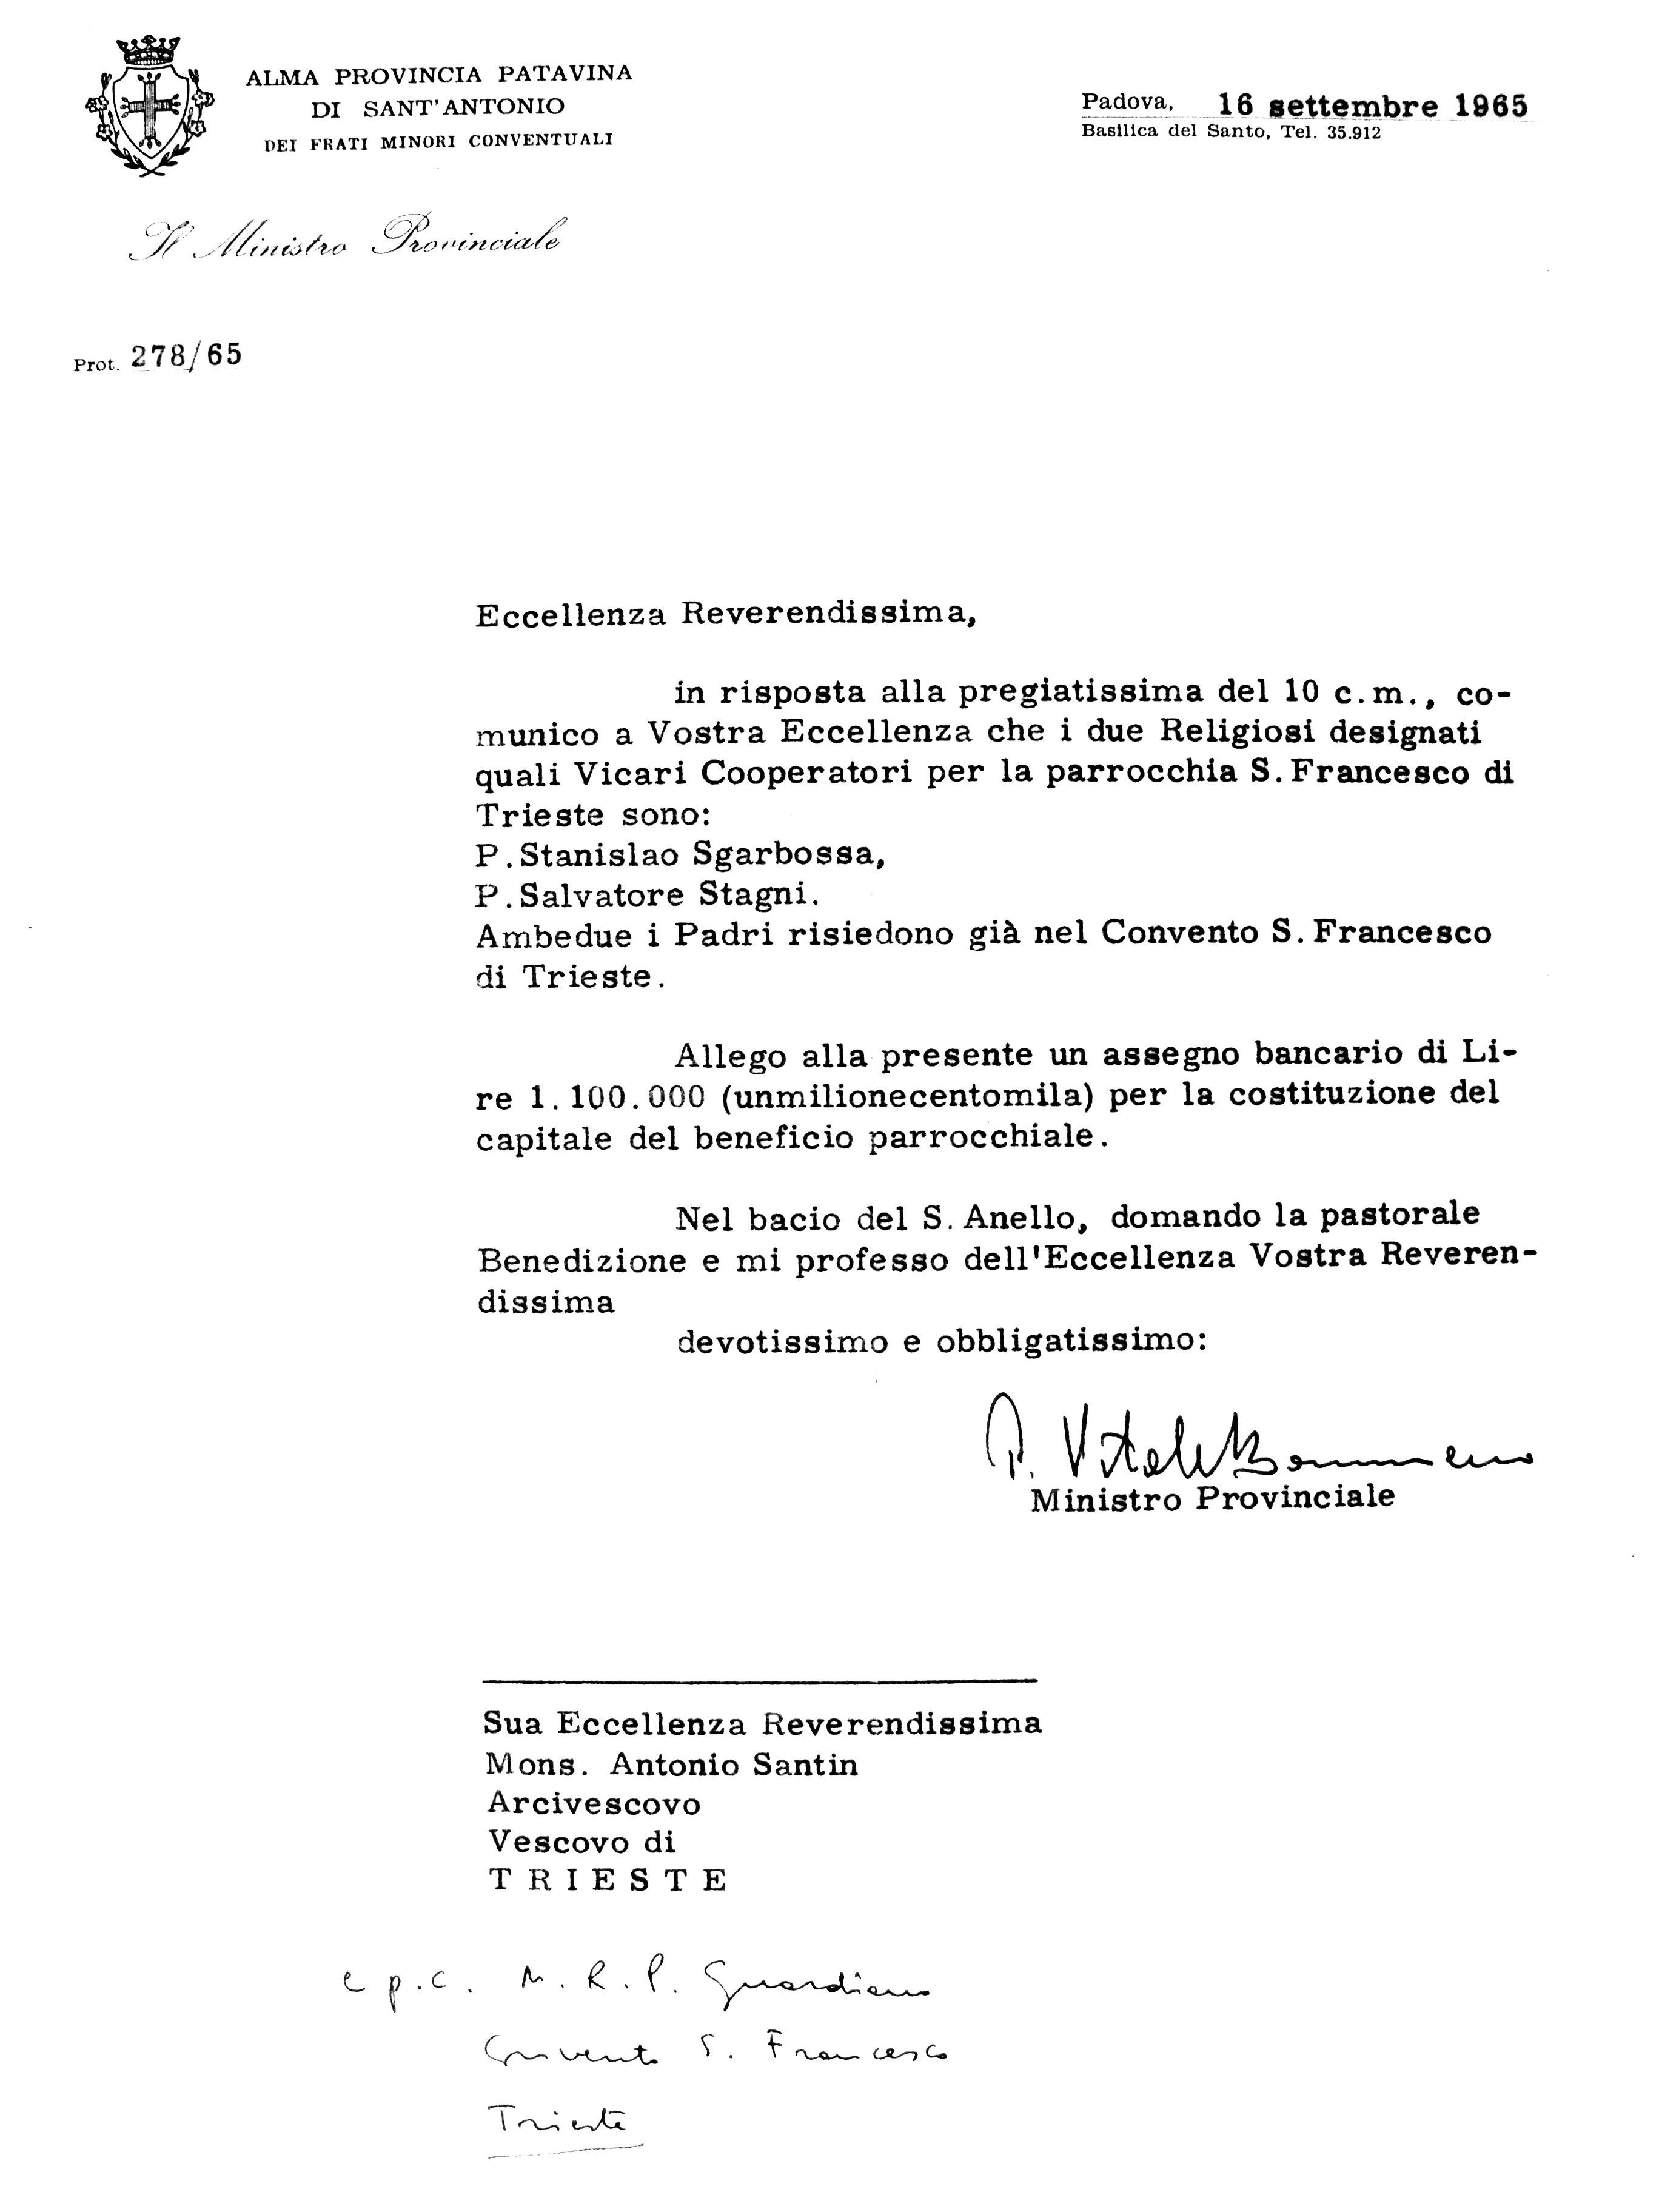
\includegraphics[
	%width=\textwidth,  
	%height=\textheight,
	%]{immagini/i_due_vicari.jpg}%
%\end{center}
%\newpage

\newpage
\begin{center}
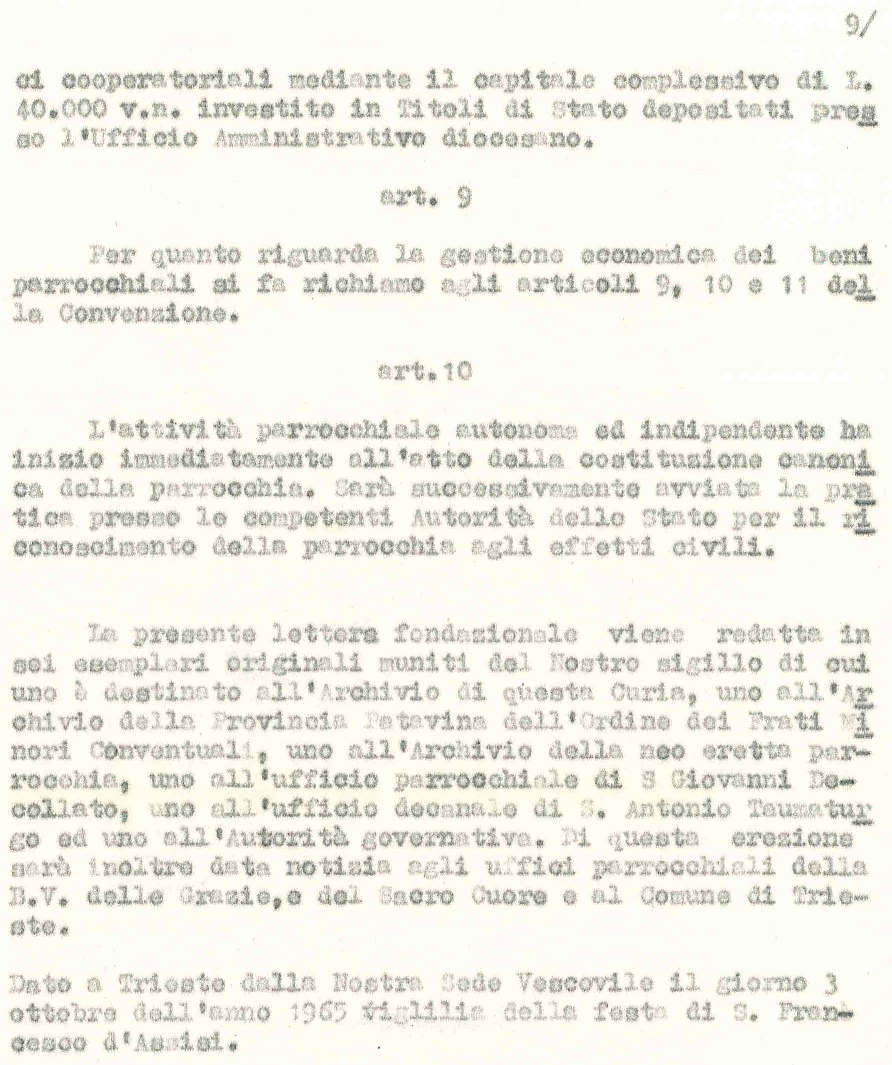
\includegraphics[
	width=1.0\textwidth
	]{testi/lettera_fondazionale10.pdf}%
\end{center}
\vspace*{10mm}
\textit{Il 3 maggio 1994 è stata rinnovata la Convenzione tra la Diocesi di Trieste e la Provincia Patavina OFM Conv (ora Provincia Italiana di S. Antonio di Padova) conforme le nuove indicazioni del Concilio Ecumenico Vaticano II.}

\newpage
\phantomsection
\addcontentsline{toc}{section}{Riconoscimento civile}
\markright{Riconoscimento civile}{}
\foreachpage{testi/riconoscimento_civile.pdf}{%
  \newpage   
  \begingroup 
    \centering
    \includegraphics[
      page=\value{imagepage},
      width=\textwidth,  
      height=\textheight,
    ]{testi/riconoscimento_civile.pdf}%
    \newpage
  \endgroup
}

\newpage
\phantomsection
\addcontentsline{toc}{section}{Saluto del Vescovo}
\markright{}{}
\begin{center}
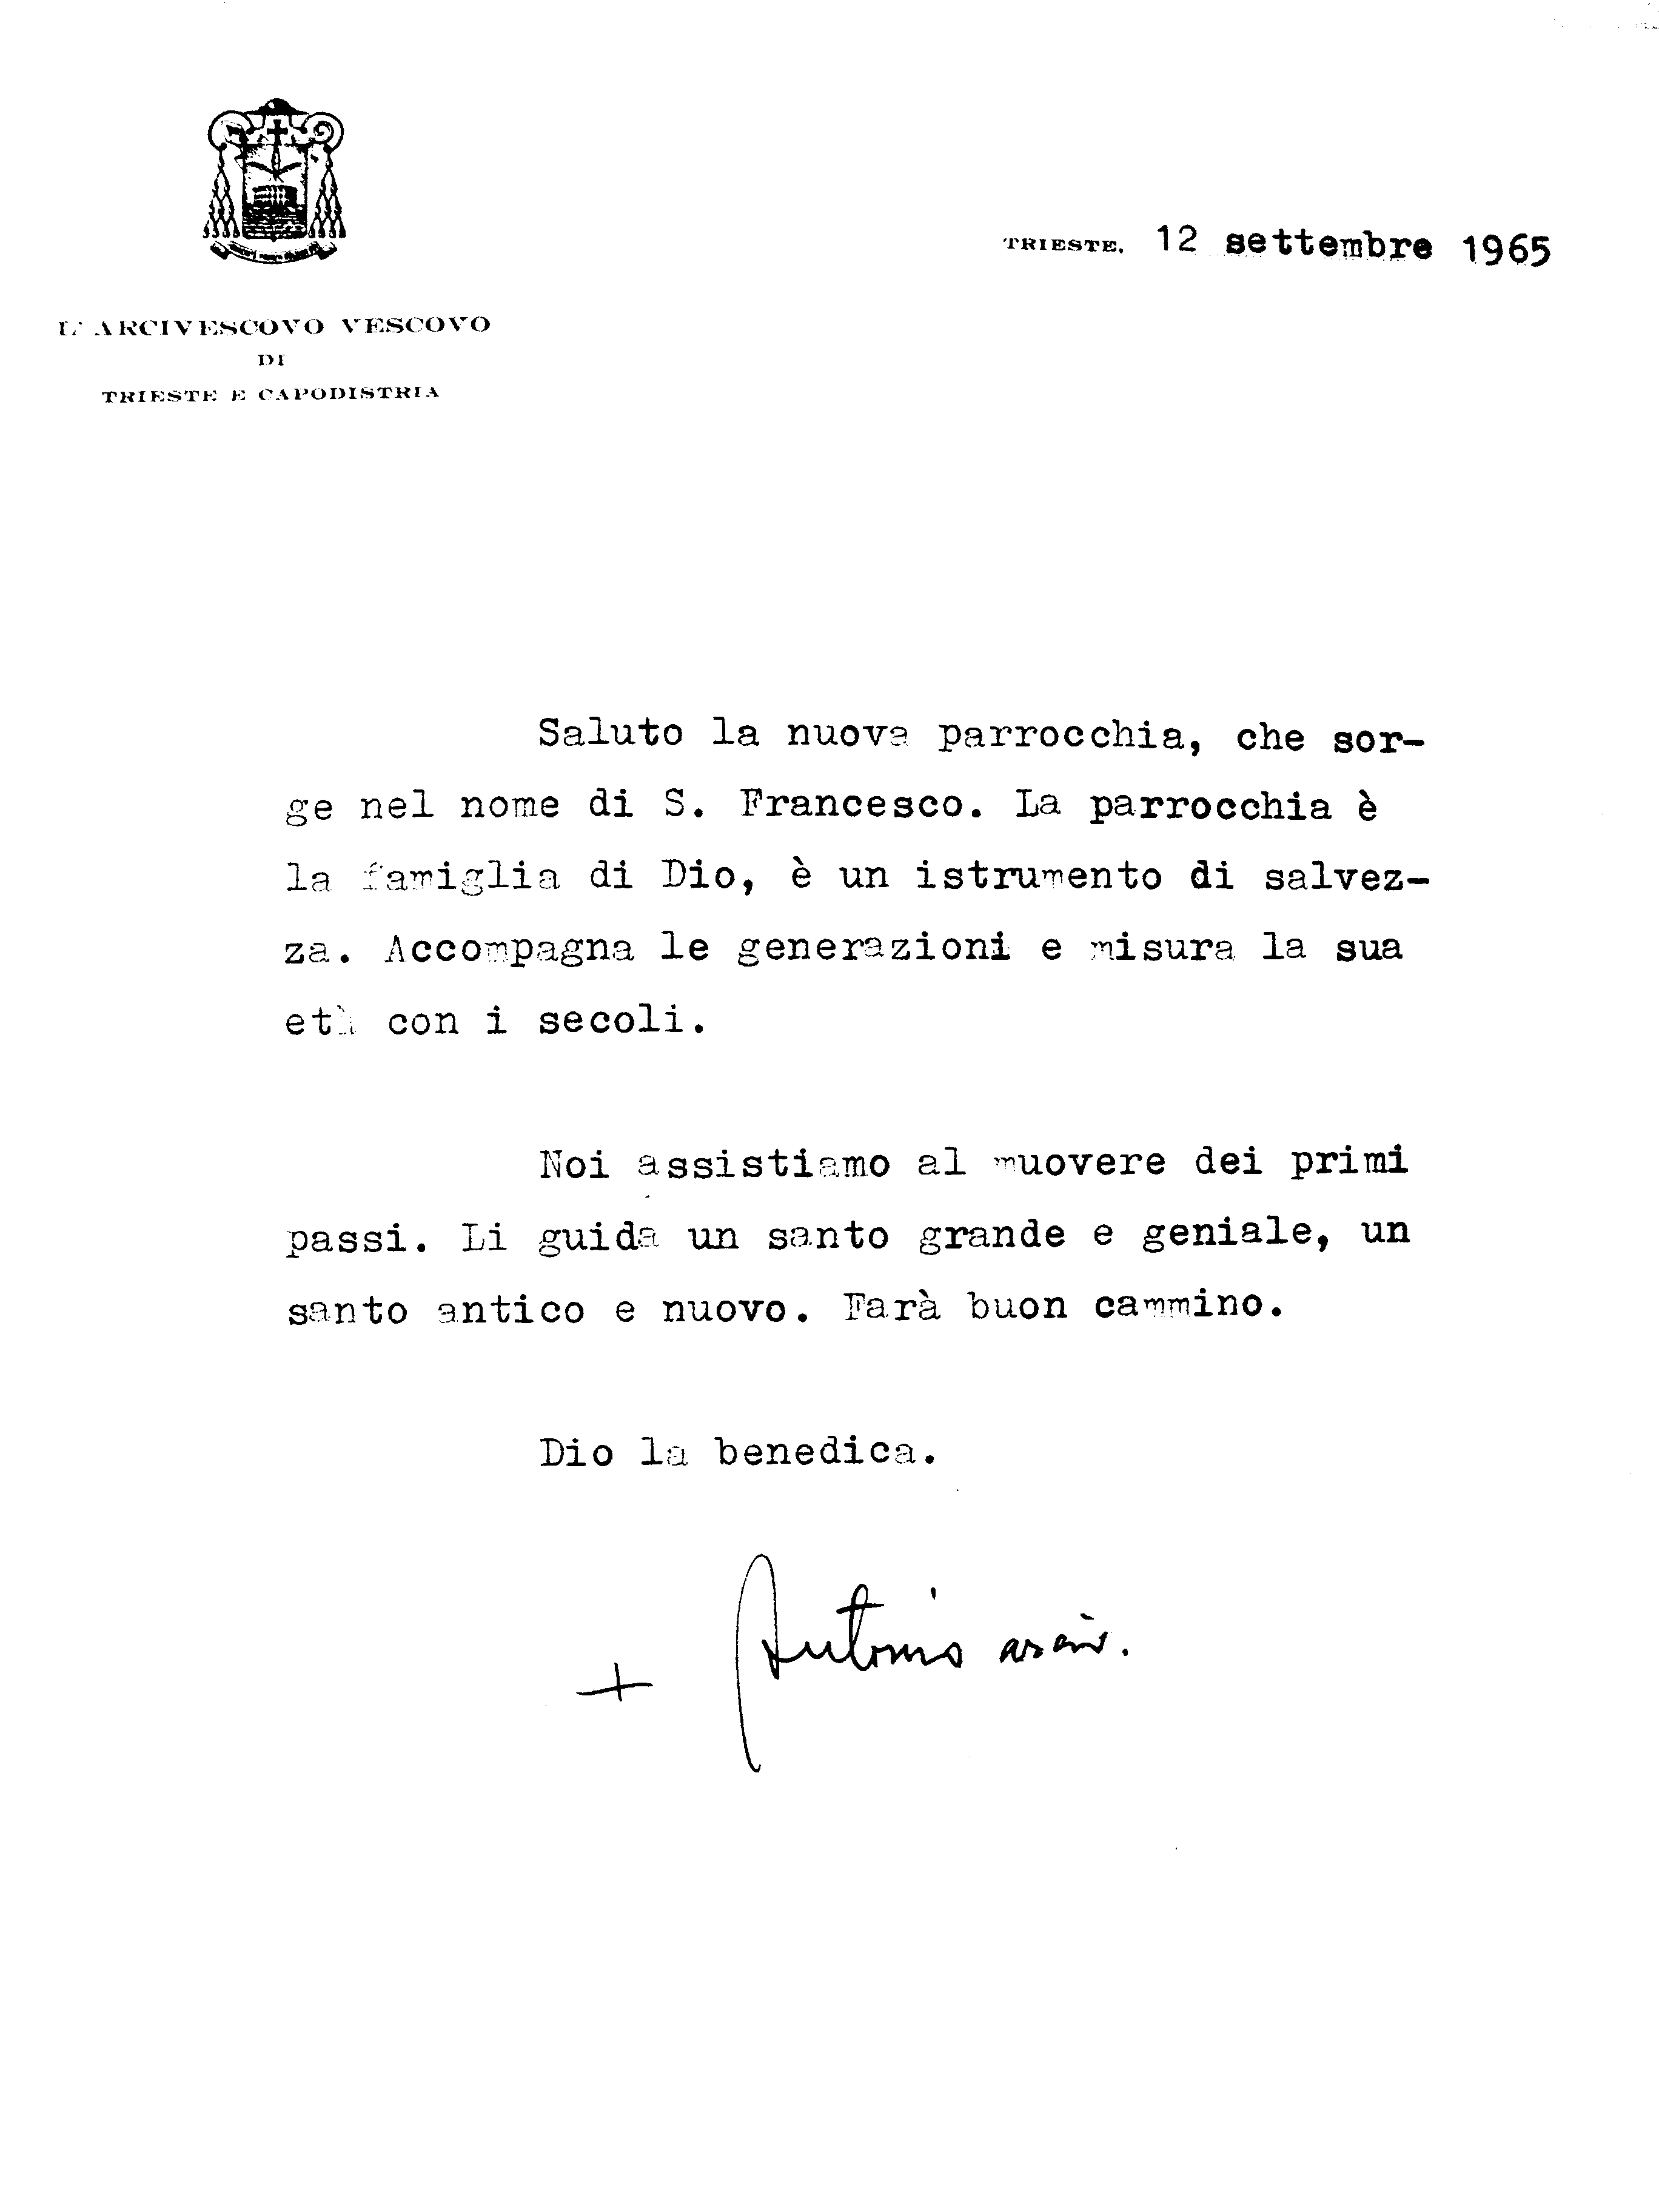
\includegraphics[
	width=\textwidth,  
	height=\textheight
	]{immagini/saluto_dal_vescovo.jpg}%
\end{center}
\newpage
\begin{center}
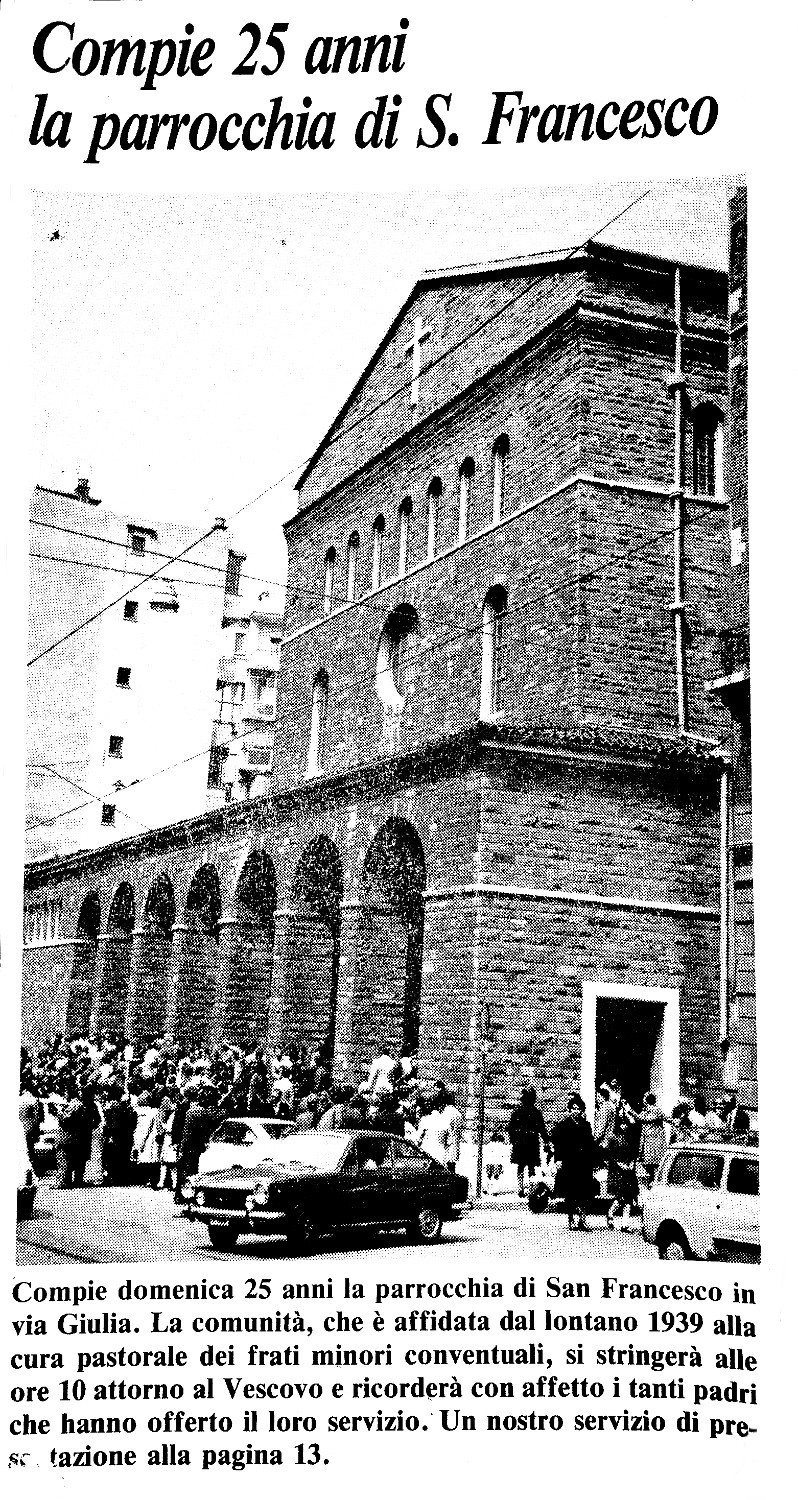
\includegraphics[
	width=\textwidth,  
	height=\textheight,
	keepaspectratio
	]{immagini/FotoParrocchia.jpg}%
\end{center}
\newpage
\begin{sidewaysfigure}
    \captionsetup{labelformat=empty}
    \centering
	  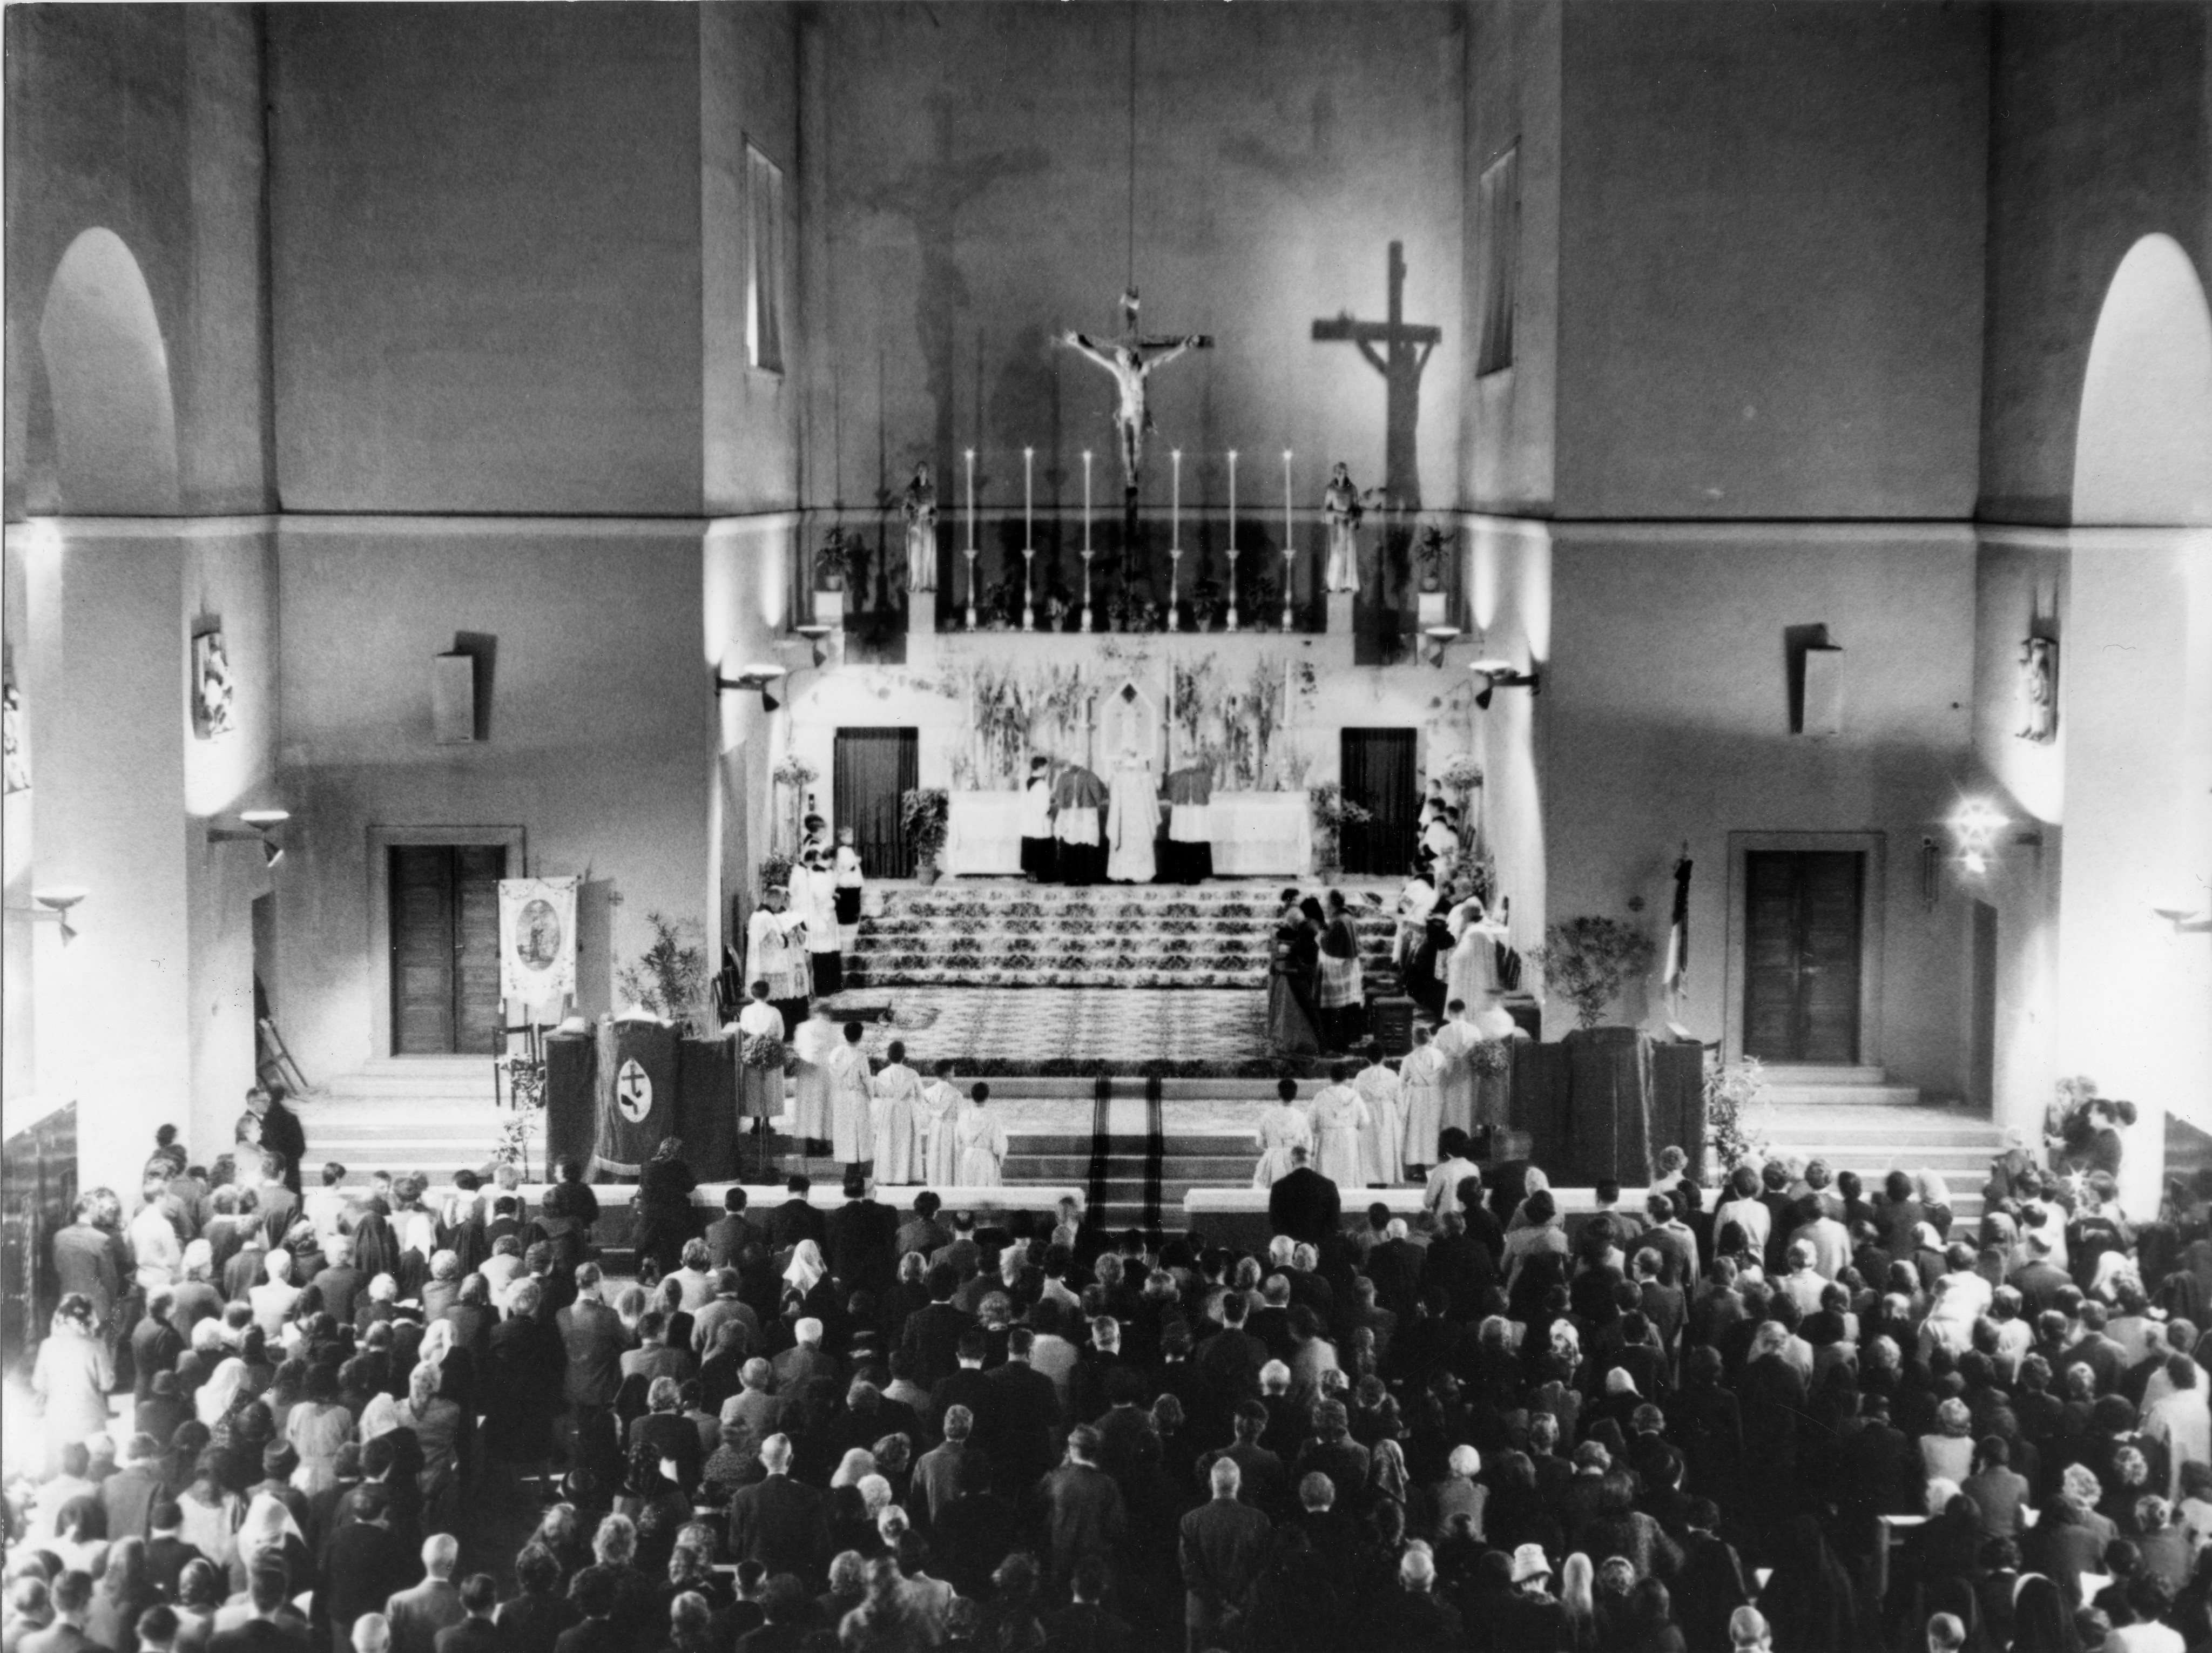
\includegraphics[width=0.85\textwidth]{immagini/Chiesa_interno.jpg}
    \caption{Veduta interna della chiesa.}
		\vspace{-15pt}
\end{sidewaysfigure}
\newpage